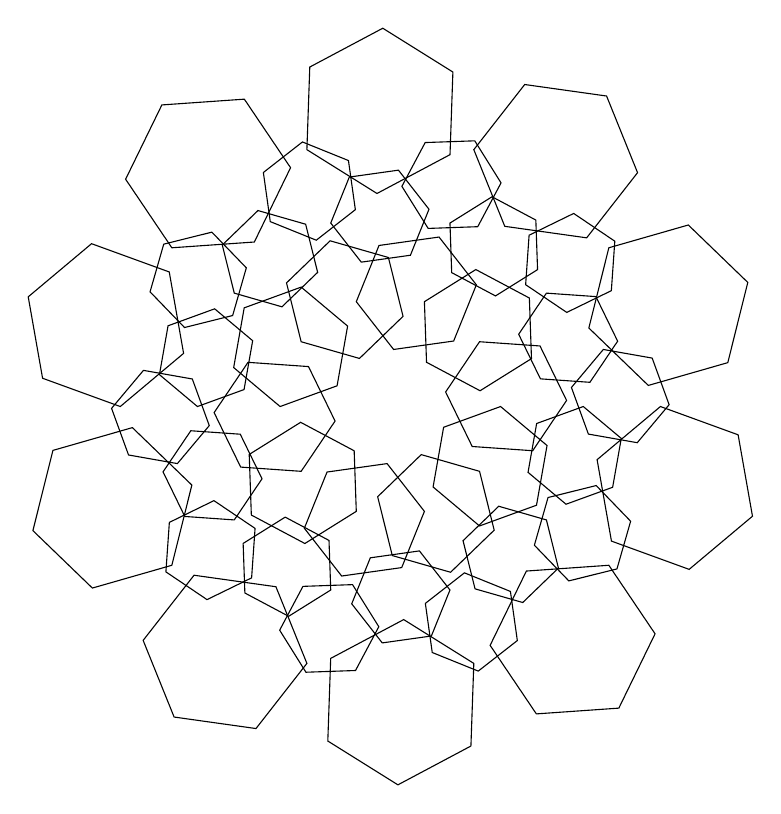
\begin{tikzpicture}[scale=.7]
    \foreach \phi in {0,36,...,324}{
        \pgfmathsetmacro{\bigHex}{1.5};
        \pgfmathsetmacro{\smallHex}{0.9};
        \pgfmathsetmacro{\leftHex}{1.1};
        \draw[rotate=\phi] (0:4.9) -- ++ (-20:\bigHex) -- ++ (-80:\bigHex) -- ++ (-140:\bigHex) -- ++ (160:\bigHex) -- ++ (100:\bigHex) -- cycle;
        \draw[rotate=\phi] (15:4) -- ++ (-10:\smallHex) -- ++ (-70:\smallHex) -- ++ (-130:\smallHex) -- ++ (170:\smallHex) -- ++ (110:\smallHex) -- cycle;
        \draw[rotate=\phi] (0:2) -- ++ (-40:\leftHex) -- ++ (-100:\leftHex) -- ++ (-160:\leftHex) -- ++ (140:\leftHex) -- ++ (80:\leftHex) -- cycle;
        \draw[rotate=\phi] (0:3.5) -- ++ (-40:\smallHex) -- ++ (-100:\smallHex) -- ++ (-160:\smallHex) -- ++ (140:\smallHex) -- ++ (80:\smallHex) -- cycle;
    }
    \end{tikzpicture}